\documentclass[sigconf]{acmart}

\usepackage{graphicx}
\usepackage{hyperref}
\usepackage{todonotes}

\usepackage{endfloat}
\renewcommand{\efloatseparator}{\mbox{}} % no new page between figures

\usepackage{booktabs} % For formal tables

\settopmatter{printacmref=false} % Removes citation information below abstract
\renewcommand\footnotetextcopyrightpermission[1]{} % removes footnote with conference information in first column
\pagestyle{plain} % removes running headers

\newcommand{\TODO}[1]{\todo[inline]{#1}}

\begin{document}
\title{Big Health Data from Wearable Electronic Sensors (WES) and 
the Treatment of Opioid Addiction}

\author{Sean M. Shiverick}
\affiliation{%
  \institution{Indiana University Bloomington}
}
\email{smshiver@indiana.edu}

%%%%%%%%%%%%%%%%%%%%%%%%%%%%%%%%%%%%%%%%%%%%%%%%%%%%%%%%%%%%%%%%%%%%%%%%%%%%%%%%%%

\begin{abstract}
Wearable electronic sensors (WES) generate to collect
vital health data in the treatment of opioid addiction. 
\end{abstract}

\keywords{Big Data Applications, Health Analytics, Wearable Sensors, i535, HID335}

\maketitle

%%%%%%%%%%%%%%%%%%%%%%%%%%%%%%%%%%%%%%%%%%%%%%%%%%%%%%%%%%%%%%%%%%%%%%%%%%%%%%%%%%

\section{Introduction}

In the increasingly connected digital age, personal electronic devices are 
generating tremendous volumes of data with important applications for 
health analytics. Wearable electronic sensors (i.e., \emph{wearables}) and
fitness monitors (e.g, FitBit, iWatch) can record our movements and vital 
physiological measures such as heart rate, temperature, and blood pressure 
\cite{metcalf16}. Consumers are using wearables to self-monitor stress 
and hypertension. In addition, wearable sensors can be used to help track
recovery following medical procedures such as surgery \cite{atallah11}. 
Emerging forms of personalized health care are arising in which individuals 
self-monitor and manage their own health in partnership with care providers.


There is currently an ongoing health crisis in the U.S. related to the abuse 
of prescription opioid medication (e.g., oxycodone, hydrocodone) that has 
grown to epidemic proportions. Approximately 2 million Americans abused or were
dependent on prescription opioids in 2014, and roughly 1 in 4 people who received
prescription opioids in primary care for non-cancer pain is struggling with 
addiction \cite{cdc17}. Overdose deaths from prescription opioids has quadrupled 
since 1999, and more than 180,000 Americans died from prescription opioid 
overdoses between 1999 to 2015 cite. Figure 1 shows that dramatic increase in 
overdose deaths in the U.S. between 2000 and 2016 are from synthetic opioids 
(other than methadone), natural and semi-synthetic opioids, and heroin 
\cite{nida17}. Of the estimated 64,000 drug overdose deaths in 2015, over 
20,000 overdose deaths were from fentanyl and other synthetic opioid analogs. 


\begin{figure}[!ht]
  \centering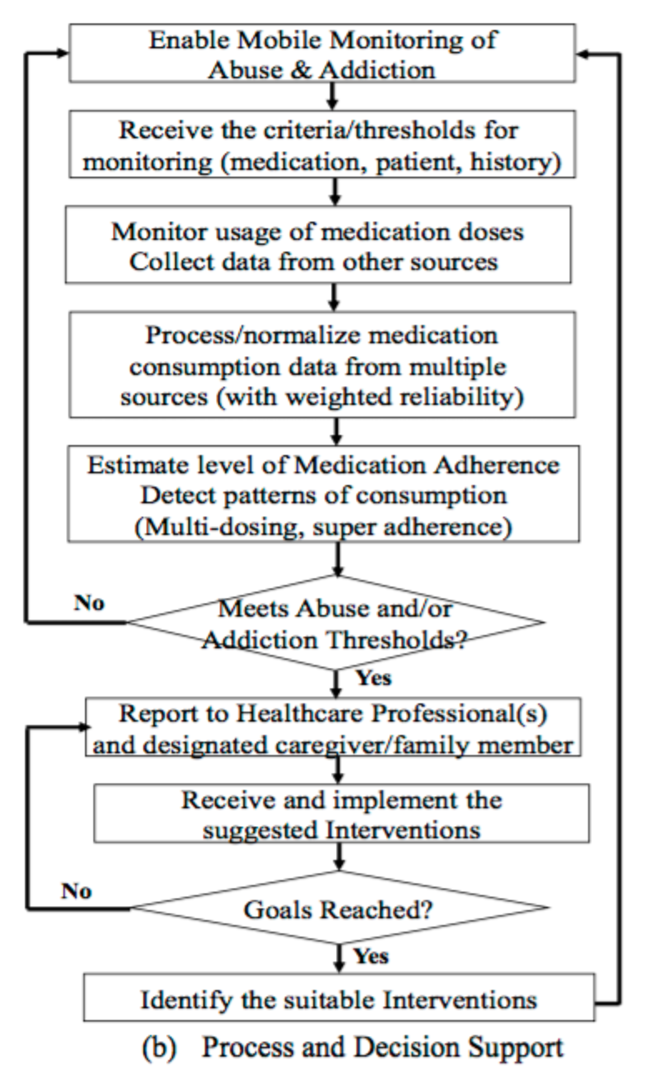
\includegraphics[width=\columnwidth]{images/Figure1.pdf}
  \caption{Drugs Involved in U.S. Overdose Deaths, 2000 to 2016 \cite{nida17}
  }\label{f:Figure1}
\end{figure}


%%%%%%%%%%%%%%%%%%%%%%%%%%%%%%%%%%%%%%%%%%%%%%%%%%%%%%%%%%%%%%%%%%%%%%%%%%%%%%%%%%
\subsection{Medication Abuse and Opioid Addiction} \cite{Varshney14}

The nature of the opioid epidemic \cite{volkow14}



%%%%%%%%%%%%%%%%%%%%%%%%%%%%%%%%%%%%%%%%%%%%%%%%%%%%%%%%%%%%%%%%%%%%%%%%%%%%%%%%%%
\subsubsection{Drug Addiction as an Illness}

For millions of people struggling with substance abuse and dependency in 
the U.S., addiction and relapse are chronic health conditions \cite{boyer10}. 
Drug addiction has many similar characteristics to other chronic medical 
illnesses; however, there are unique challenges to the treatment of addiction
illnesses. For example, drug addicted patients undergo intense detoxification 
in rehabilitation treatment programs, but then are released back into the same 
environment associated with their drug use. The lack of continuity in the 
treatment of addiction disorders, leaves addicts in recovery at high risk for
relapse into substance use and abuse. Second, individuals with addiction 
disorders present for care to emergency rooms after acute intoxication, often 
following law enforcement interventions. Emergency personal and very capable 
at crisis intervention for drug overdose, but lack resources to evaluate severe 
addiction disorders or provide follow-up. Furthermore, addicted individuals 
seeking treatment often relapse at night or on weekends when treatment centers 
are not open. Various theories of addiction and relapse have been proposed. 
According to the classical conditioning model, situational cues or events can 
elicit a motivational state underlying relapse to drug use. A slightly more 
complex model suggests that addictive behavior can be reinstated after 
extinction of dependency by exposure to drugs, drug-related cues, or 
environmental stressors \cite{shaham03}. Understanding that a user`s affective
response to cues in the environmental can lead to relapse and drug use are key 
to developing strategies for prevention and treatment. 


%%%%%%%%%%%%%%%%%%%%%%%%%%%%%%%%%%%%%%%%%%%%%%%%%%%%%%%%%%%%%%%%%%%%%%%%%%%%%%%%%%
\subsection{Review of Technology-Based Interventions for Addiction Treatment}

Technology-based interventions have been used for drug addiction assessment, 
treatment, prevention and recovery \cite{marsch12}. In terms of assessment, data 
about individuals substance use can be obtained from mobile cell phone reporting 
outside of treatment settings. Web-based approaches to treatment have been 
implemented online to improve behavioral and psychosocial functioning for addicted 
individuals in recovery \cite{marschdallery2012}. For example, the Therapeutic 
Education System (TES) is a self-directed, web-based interactive treatment program 
consisted of 65 training modules that  focuses cognitive-behavioral skills, 
psychosocial functioning (family/social relations). This online approach helped 
to increase access to treatment for individuals in rural areas, and included an 
optional contingency management module. A computer based Training in Cognitive 
Behavioral Therapy (CBT) program was found to enhance treatment outcomes when 
provided in conjunction with traditional substance abuse treatment, and helped 
improve coping skills and decision-making skills \cite{carroll08}. In evaluating 
the effectiveness of mobile applications for addiction treatment, several  
questions remain to be answered: First, if mobile applications primarily are
regarded primarily as supplements to traditional therapeutic treatment, can their 
effectiveness be measured independently from the approach used in treatment? 
Second, over what time period period can the benefits of mobile applications be 
observed? Research evidence suggests that the benefits of mobile interventions 
may be limited to 12 or 15 weeks \cite{swedenson16}. However, it is unclear 
whether individuals struggling from addiction would continue to use mobile 
treatment applications in the long terms, beyond a limited course of treatment.


%%%%%%%%%%%%%%%%%%%%%%%%%%%%%%%%%%%%%%%%%%%%%%%%%%%%%%%%%%%%%%%%%%%%%%%%%%%%%%%%%%
\subsubsection{Mobile-Based Applications for Addiction Treatment}

Mobile based applications have been used for monitoring and treatment of 
substance abuse and addiction disorders for several decades \cite{boyer10}. 
Early applications included the use of electronic pagers (i.e., beepers) 
for experience sampling with paper-based assessments that generated data about 
daily life behavior and experiences \cite{swedenson16}. In the 1990s, programmable 
personal digital assistants (i.e., palm-pilot) enabled collection of data 
electronically, and subsequent mobile research tools facilitated the collection 
of information about psychological factors (e.g., daily stressors, emotional 
states, thoughts) and other variables related to addiction (e.g., craving, 
contextual cues, actual substance use). Assessments performed several times 
throughout the day (commonly, every 2 to 4 hours) allowed for analysis of the 
daily fluctuations of these symptoms and features. Historically, addiction 
research has faced some unique challenges that the use of mobile technologies 
may help to overcome. Methodological aspects of traditional research using 
retrospective, cross-sectional, or longitudinal assessments (over periods of 
weeks, months, or years) have been problematic for investigating risk factors 
including behaviors and symptoms (severe physiological cravings, withdrawal, 
and substance use) that can span a relatively short time. An additional factor 
is the comorbidity, or co-occurence, of substance use disorders (SUDs) with other 
psychological disorders, such as anxiety and mood disorders. For example, the 
``self-medication’’ model has commonly been used to explain the association 
between alcohol abuse is used as an effort by an individual to reduce or cope 
with a high degree of anxiety (or depression). It has also been challenging 
for researchers to capture the role of environmental or contextual cues (e.g., 
people, places, things) associated with substance abuse and addiction, which 
can trigger relapse for individuals in recovery.


%%%%%%%%%%%%%%%%%%%%%%%%%%%%%%%%%%%%%%%%%%%%%%%%%%%%%%%%%%%%%%%%%%%%%%%%%%%%%%%%%%
\subsubsection*{Smartphone Application for Addiction and recovery}

Continued care is an important ingredient for recovery from addiction that
involves monitoring, outreach, planning, case management, and social support 
\cite{johnson11}. Smartphone applications can help individuals in recovery to 
monitor cravings at critical points in daily life, track contextual cues 
associated with substance use, and provide outreach to support services. A team 
of researchers at the University of Wisconsin evaluated the effectiveness of a
smartphone application called Addiction Comprehensive Health Enhancement Support 
System (A-CHESS), designed to provide recovery support patients leaving 
residential alcohol treatment center \cite{gustafson14}. A-CHESS provided anytime, 
anywhere access to support services in audio-visual format, GPS monitoring and 
warnings for risky locations, and communication with counselors. Over an 8-month
period and 4 month follow-up, patients who used the A-CHESS intervention reported
fewer risky drinking days, on average, per month than patients in a comparable
control group. The findings provide evidence that the smartphone intervention was 
effective at treating a critical behavioral measure for treatment of alcohol use 
disorder (AUD). 


%%%%%%%%%%%%%%%%%%%%%%%%%%%%%%%%%%%%%%%%%%%%%%%%%%%%%%%%%%%%%%%%%%%%%%%%%%%%%%%%%%
\subsection{Wearable Sensors}

Many smartphones have built-in sensors (accelerometer, odometer, GPS) that can 
track movement and activity. Although not specifically designed to collect
clinical data, smartphone sensors can be repurposed help addicted individuals 
to track signs of  potential relapse. Additional sensors could be added to a 
smartphone to monitor heart rate, respiration, and body temperature and 
communicate physiological data to care providers or treatment specialists to
provide support or initiate an intervention if necessary \cite{johnson11}. 
GPS coordinates can be used to monitor proximity to locations or persons 
associated with substance use


Real-Time Mobile Detection of Drug Use with Wearable Biosensors:
A Pilot Study
\cite{carreiro15}

%%%%%%%%%%%%%%%%%%%%%%%%%%%%%%%%%%%%%%%%%%%%%%%%%%%%%%%%%%%%%%%%%%%%%%%%%%%%%%%%%%
\subsection{Emerging Technologies}

%%%%%%%%%%%%%%%%%%%%%%%%%%%%%%%%%%%%%%%%%%%%%%%%%%%%%%%%%%%%%%%%%%%%%%%%%%%%%%%%%%
\subsubsection{Tattoo sensors}

If you like to see a more elaborate example, please look at
report-long.tex. 


%%%%%%%%%%%%%%%%%%%%%%%%%%%%%%%%%%%%%%%%%%%%%%%%%%%%%%%%%%%%%%%%%%%%%%%%%%%%%%%%%%
\subsubsection{LoRa Backscatter}

If you like to see a more elaborate example, please look at
report-long.tex. 


%%%%%%%%%%%%%%%%%%%%%%%%%%%%%%%%%%%%%%%%%%%%%%%%%%%%%%%%%%%%%%%%%%%%%%%%%%%%%%%%%%
\subsection{Effectiveness of Technology-Based Interventions Addiction Treatment and Recovery}


\section{figures}

%In Figure \ref{f:fly} we show a fly. Please note that because we use
just columwidth that the size of the figure will change to the
columnwidth of the paper once we change the layout to final. CHnaging
the layout to final should not be done by you. All figures will be
listed at the end.

%\begin{figure}[!ht]
%  \centering\includegraphics[width=\columnwidth]{images/fly.pdf}
%  \caption{Example caption}\label{f:fly}
%\end{figure}

When copying the example, please do not check in the images from the
examples into your images directory as you will not need them for your
paper. Instead use images that you like to include. If you do not have
any images, do not dreate the images folder.

\section{Tables}

In case you need to create tables, you can do this with online tools
(if you do not mind sharing your data) such as
%\url{https://www.tablesgenerator.com/} or other such tools (please
google for them). They even allow you to manage tables as CSV.

%or generate them by hand while using the provided template in 
%Table\ref{t:mytable}. 
Note that the caption is before the tabular environment.

%\begin{table}[htb]
%\centering
%\caption{My caption}
%\label{t:mytabble}
%\begin{tabular}{lll}
%1 & 2 & 3 \\
%\hline
%4 & 5 & 6 \\
%7 & 8 & 9
%\end{tabular}
%\end{table}

\section{Long example}

If you like to see a more elaborate example, please look at
report-long.tex. 

\section{Conclusion}

Put here an conclusion. Conlcusions and abstracts must not have any
citations in the section.


\begin{acks}

  The authors would like to thank Dr. Gregor von Laszewski for his
  support and suggestions to write this paper.

\end{acks}

\bibliographystyle{ACM-Reference-Format}
\bibliography{report} 

\appendix

We include an appendix with common issues that we see when students
submit papers. One particular important issue is not to use the
underscore in bibtex labels. Sharelatex allows this, but the
proceedings script we have does not allow this.

When you submit the paper you need to address each of the items in the
issues.tex file and verify that you have done them. Please do this
only at the end once you have finished writing the paper. To d this
cange TODO with DONE. However if you check something on with DONE, but
we find you actually have not executed it correcty, you will receive
point deductions. Thus it is important to do this correctly and not
just 5 minutes before the deadline. It is better to do a late
submission than doing the check in haste. 

%\section{Issues}

\DONE{Example of done item: Once you fix an item, change TODO to DONE}

\subsection{Assignment Submission Issues}

    \DONE{Do not make changes to your paper during grading, when your repository should be frozen.}

\subsection{Uncaught Bibliography Errors}

    \DONE{Missing bibliography file generated by JabRef}
    \DONE{Bibtex labels cannot have any spaces, \_ or \& in it}
    \DONE{Citations in text showing as [?]: this means either your report.bib is not up-to-date or there is a spelling error in the label of the item you want to cite, either in report.bib or in report.tex}

\subsection{Formatting}

    \DONE{Incorrect number of keywords or HID and i523 not included in the keywords}
    \DONE{Other formatting issues}

\subsection{Writing Errors}

    \DONE{Errors in title, e.g. capitalization}
    \DONE{Spelling errors}
    \DONE{Are you using {\em a} and {\em the} properly?}
    \DONE{Do not use phrases such as {\em shown in the Figure below}. Instead, use {\em as shown in Figure 3}, when referring to the 3rd figure}
    \DONE{Do not use the word {\em I} instead use {\em we} even if you are the sole author}
    \DONE{Do not use the phrase {\em In this paper/report we show} instead use {\em We show}. It is not important if this is a paper or a report and does not need to be mentioned}
    \DONE{If you want to say {\em and} do not use {\em \&} but use the word {\em and}}
    \DONE{Use a space after . , : }
    \DONE{When using a section command, the section title is not written in all-caps as format does this for you}\begin{verbatim}\section{Introduction} and NOT \section{INTRODUCTION} \end{verbatim}

\subsection{Citation Issues and Plagiarism}

    \DONE{It is your responsibility to make sure no plagiarism occurs. The instructions and resources were given in the class}
    \DONE{Claims made without citations provided}
    \DONE{Need to paraphrase long quotations (whole sentences or longer)}
    \DONE{Need to quote directly cited material}

\subsection{Character Errors}

    \DONE{Erroneous use of quotation marks, i.e. use ``quotes'' , instead of " "}
    \DONE{To emphasize a word, use {\em emphasize} and not ``quote''}
    \DONE{When using the characters \& \# \% \_  put a backslash before them so that they show up correctly}
    \DONE{Pasting and copying from the Web often results in non-ASCII characters to be used in your text, please remove them and replace accordingly. This is the case for quotes, dashes and all the other special characters.}
    \DONE{If you see a figure and not a figure in text you copied from a text that has the fi combined as a single character}

\subsection{Structural Issues}

    \DONE{Acknowledgement section missing}
    \DONE{Incorrect README file}
    \DONE{In case of a class and if you do a multi-author paper, you need to add an appendix describing who did what in the paper}
    \DONE{The paper has less than 2 pages of text, i.e. excluding images, tables and figures}
    \DONE{The paper has more than 6 pages of text, i.e. excluding images, tables and figures}
    \DONE{Do not artificially inflate your paper if you are below the page limit}

\subsection{Details about the Figures and Tables}

    \DONE{Capitalization errors in referring to captions, e.g. Figure 1, Table 2}
    \DONE{Do use {\em label} and {\em ref} to automatically create figure numbers}
    \DONE{Wrong placement of figure caption. They should be on the bottom of the figure}
    \DONE{Wrong placement of table caption. They should be on the top of the table}
    \DONE{Images submitted incorrectly. They should be in native format, e.g. .graffle, .pptx, .png, .jpg}
    \DONE{Do not submit eps images. Instead, convert them to PDF}

    \DONE{The image files must be in a single directory named "images"}
    \DONE{In case there is a powerpoint in the submission, the image must be exported as PDF}
    \DONE{Make the figures large enough so we can read the details. If needed make the figure over two columns}
    \DONE{Do not worry about the figure placement if they are at a different location than you think. Figures are allowed to float. For this class, you should place all figures at the end of the report.}
    \DONE{In case you copied a figure from another paper you need to ask for copyright permission. In case of a class paper, you must include a reference to the original in the caption}
    \DONE{Remove any figure that is not referred to explicitly in the text (As shown in Figure ..)}
    \DONE{Do not use textwidth as a parameter for includegraphics}
    \DONE{Figures should be reasonably sized and often you just need to
  add columnwidth} e.g. \begin{verbatim}/includegraphics[width=\columnwidth]{images/myimage.pdf}\end{verbatim}

re


\end{document}
